\chapter{Computational results}
The algorithm was implemented using Python 3, tensorflow 2.9.1 and scipy 1.9.3. In this part we compare our proposed solver to the state-of-art ReduMIS solver.
Tests include search of the MIS on generated graphs and on DIMACS graphs. All results are compared to the state-of-art ReduMIS algorithm built with GNU C++ in terms of accuracy and execution time. Tests are executed on Intel(R) Core(TM) i7-6700HQ CPU @ 2.60GHz in single thread.

\subsection{Generated graphs results}
We test network on randomly generated higher-density graphs using from the Erdos-Renyi (ER) \cite{er60}, Barbosi-Albert (BA) \cite{ab02}, Holme and Kim (HK) \cite{hk02}, and the Stochastic Block (SBM) \cite{hll83} models.

\begin{table}[!ht]
    \centering
    \begin{tabular}{|l|l|l|l|l|l|}
    \hline
        \textbf{Graph} & \textbf{V} & \textbf{E} & \textbf{dNN result} & \textbf{ReduMIS result} & \textbf{Accuracy} \\ \hline
        \textbf{ER} & 100 (p = 0.1) & 500,00 & 28,15 & 30,50 & 0,92295082 \\ \hline
        \textbf{ER} & 100  (p = 0.2) & 983,00 & 18,00 & 20,00 & 0,9 \\ \hline
        \textbf{ER} & 200  (p = 0.1) & 2004,00 & 35,90 & 41,00 & 0,875609756 \\ \hline
        \textbf{ER} & 200  (p = 0.2) & 4000,00 & 20,00 & 25,50 & 0,784313725 \\ \hline
        \textbf{SBM} & 250  (p = 0.1) & 1874,00 & 55,50 & 61,00 & 0,909836066 \\ \hline
        \textbf{SBM} & 250  (p = 0.2) & 2481,00 & 45,90 & 51,00 & 0,9 \\ \hline
        \textbf{SBM} & 350  (p = 0.1) & 3666,00 & 63,10 & 68,00 & 0,927941176 \\ \hline
        \textbf{SBM} & 350  (p = 0.2) & 4883,00 & 51,60 & 55,50 & 0,92972973 \\ \hline
        \textbf{BA} & 100 & 2475,00 & 45,00 & 45,00 & 1 \\ \hline
        \textbf{BA} & 200 & 9950,00 & 95,00 & 95,00 & 1 \\ \hline
        \textbf{HK} & 100 & 2017,00 & 30,00 & 30,00 & 1 \\ \hline
        \textbf{HK} & 200 & 8092,00 & 60,00 & 60,00 & 1 \\ \hline
    \end{tabular}
    \caption{Dataless neural network result comparison with state-of-art ReduMIS solver}
    \label{table:generated_graphs_result}
\end{table}

For testing we also use DIMACS benchmark. The 1990s saw the creation of the DIMACS benchmark set for the second DIMACS challenge on Clique, Satisfiability, and Graph Coloring (Johnson \& Trick, 1996). It consists of 80 graphs and is the benchmark set for assessing MCP algorithms. The benchmark includes several real-world issues, including coding theory, fault diagnosis issues, Keller's hypothesis, and others, in addition to randomly generated networks and graphs in which the largest clique is concealed by using low-degree vertices.

On the figure \ref{fig:heuristic_algorithms_description} we can see description of the some most efficient heurstic algorithms for the MIS problem. On the table \ref{table:heuristic_algorithms_results} and \ref{table:heuristic_algorithms_performance} the average accuracy and performance of these algorithms is presented for the MIS problem on DIMACS graphs.
\begin{figure}[h]
    \centering
    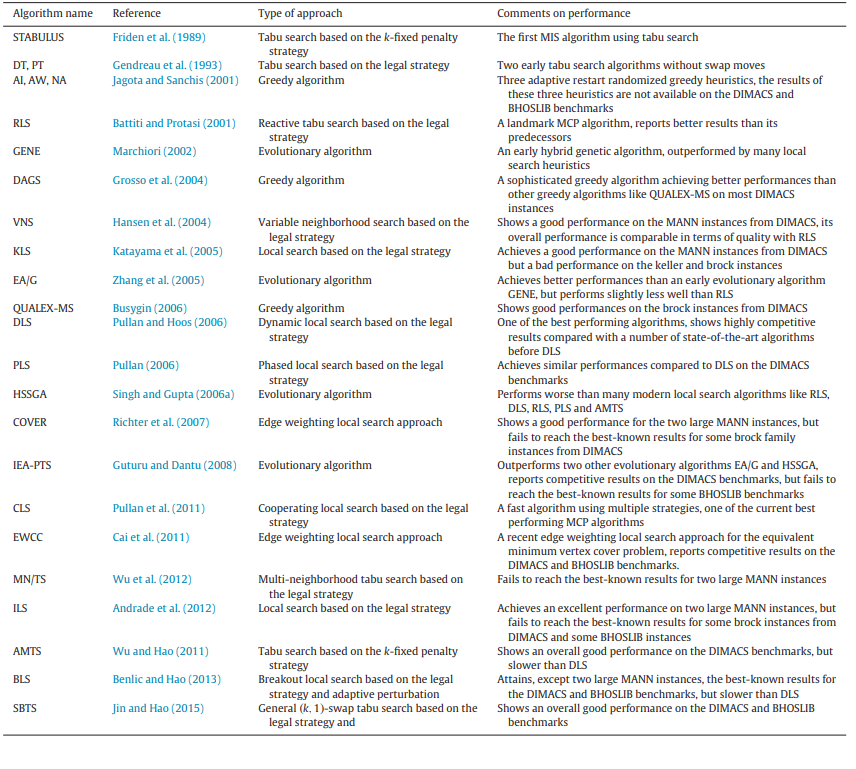
\includegraphics{figures/heuristic_algorithms_description.png}
    \caption{Best existing heuristic algorithms for MIS problem with description}
    \label{fig:heuristic_algorithms_description}
\end{figure}

\begin{table}[!ht]
    \centering
    \begin{tabular}{|l|l|l|l|l|l|l|}
    \hline
        \textbf{Instance} & \textbf{brock400\_2} & \textbf{brock800\_2} & \textbf{C2000.9} & \textbf{C4000.5} & \textbf{keller6} & \textbf{MANN\_a81} \\ \hline
        \textbf{RLS} & 29(26.06) & 21 & 78(77.58) & 18 & 59 & 1098 \\ \hline
        \textbf{GENE} & 24(22.5) & 20(19.3) & 72(68.2) & 16(15.4) & 55(51.8) & 1097(1096.3) \\ \hline
        \textbf{DAGS} & 29(28.10) & 24(20.82) & 76(75.40) & 18(17.50) & 57(56.40) & ~ \\ \hline
        \textbf{VNS} & 29(27.4) & 21 & 78(77.2) & 18 & 59(58.2) & 1100(1099.3) \\ \hline
        \textbf{KLS} & 25(24.84) & 21(20.86) & 77(74.90) & 18(17.02) & 57(55.59) & 1100(1098.07) \\ \hline
        \textbf{EA/G} & 25(24.7) & 21(20.1) & 72(70.9) & 17(16.1) & 56(53.4) & 1098(1097.2) \\ \hline
        \textbf{QUALEX-MS} & 29 & 24 & 72 & 17 & 53 & 1096 \\ \hline
        \textbf{DLS} & 29 & 24 & 78(77.93) & 18 & 59 & 1098(1097.96) \\ \hline
        \textbf{PLS} & 29 & 24 & 78 & 18 & 59(57.75) & 1098 \\ \hline
        \textbf{HSSGA} & 29(25.1) & 21(20.7) & 74(71.0) & 17(16.8) & 57(54.2) & 1095(1094.2) \\ \hline
        \textbf{COVER} & 28(-) & - & 78(77.84) & 18 & 59 & 1100(-) \\ \hline
        \textbf{IEA-PTS} & 29(27.52) & 24(21.06) & 79(76.4) & 18(17.66) & 59(57.06) & 1099(1097.01) \\ \hline
        \textbf{CLS} & 29 & 24 & 78 & 18 & 59 & 1098 \\ \hline
        \textbf{EWCC} & 29(25.48) & 21 & 79(78.56) & 18 & 59 & 1100(1098.11) \\ \hline
        \textbf{MN/TS} & 29 & 24(23.88) & 80(78.37) & 18 & 59 & 1090 \\ \hline
        \textbf{ILS} & 25 & 21 & 77(76.9) & 18(17.1) & 59 & 1100 \\ \hline
        \textbf{AMTS} & 29 & 24 & 80(78.95) & 18 & 59 & 1098 \\ \hline
        \textbf{BLS} & 29 & 24(23.04) & 80(78.6) & 18 & 59 & 1094(1092.17) \\ \hline
        \textbf{SBTS} & 29 & 24(22.29) & 80(77.29) & 18 & 59 & 1100 \\ \hline
    \end{tabular}
    \caption{Best and average results on the heuristic algorithms for MIS problem on DIMACS graphs}
    \label{table:heuristic_algorithms_results}
\end{table}

\begin{table}[!ht]
    \centering
    \begin{tabular}{|l|l|l|l|l|l|l|}
    \hline
        \textbf{Instance} & \textbf{brock400\_2} & \textbf{brock800\_2} & \textbf{C2000.9} & \textbf{C4000.5} & \textbf{MANN\_a81} & \textbf{keller6} \\ \hline
        \textbf{RLS} & 3.06 & 0.34 & 59.83 & 158.65 & 205.72 & 13.7 \\ \hline
        \textbf{GENE} & 0.27 & 0.75 & 4.89 & 1.95 & 401.41 & 8.7 \\ \hline
        \textbf{DAGS} & 0.62 & 3.73 & 405.33 & 717.55 & - & 2739.1 \\ \hline
        \textbf{VNS} & 4.17 & 0.85 & 22.74 & 310.71 & 65.47 & 17.9 \\ \hline
        \textbf{KLS} & 0.04 & 0.16 & 4.80 & 7.76 & 12.88 & 17,0 \\ \hline
        \textbf{EA/G} & 1.42 & 3.42 & 17.38 & 23.46 & 319.04 & 24.2 \\ \hline
        \textbf{QUALEX-MS} & 0.67 & 4.00 & 47.78 & 521.11 & 106.00 & 286.8 \\ \hline
        \textbf{DLS} & 0.12 & 3.97 & 48.79 & 45.76 & 66.66 & 43.0 \\ \hline
        \textbf{PLS} & 0.12 & 4.08 & 50.11 & 47.01 & 172.17 & 172.1 \\ \hline
        \textbf{HSSGA} & 0.14 & 1.35 & 14.83 & 19.97 & 503.99 & 39.6 \\ \hline
        \textbf{COVER} & - & ~ & 139.36 & 260.27 & - & 5.8 \\ \hline
        \textbf{IEA-PTS} & 1.08 & 1.03 & 19.71 & 104.21 & 237.55 & 45.4 \\ \hline
        \textbf{CLS} & 0.08 & 1.73 & 7.28 & 13.63 & 20.80 & 0.9 \\ \hline
        \textbf{EWCC} & 374.52 & 0.49 & 858.73 & 738.91 & 634.46 & 3.7 \\ \hline
        \textbf{MN/TS} & 0.81 & 94.25 & 339.57 & 86.96 & 380.87 & 58.9 \\ \hline
        \textbf{ILS} & 11.57 & 63.15 & 108.42 & 1996.84 & 10.52 & 546.3 \\ \hline
        \textbf{AMTS} & 0.69 & 19.61 & 266.33 & 74.93 & 16.30 & 6.3 \\ \hline
        \textbf{BLS} & 10.29 & 637.94 & 2846.84 & 387.33 & - & 14.6 \\ \hline
        \textbf{SBTS} & 11.97 & 464.12 & 896.78 & 919.07 & 13.43 & 446.6 \\ \hline
    \end{tabular}
    \caption{Heuristic algorithms time performance (in seconds) on DIMACS graphs}
    \label{table:heuristic_algorithms_performance}
\end{table}

TODO: Add evolutionary minimization/gradient comparison.